% arara: xelatex: {synctex: true}
% arara: indent: {overwrite: yes}
\documentclass[]{IMTexam}

\usepackage{IMTtikz}

\givecredits
\author{Isabella B.}
\USPN{11810773}
\date{}
\lecture{Física I} % disciplina
\lcode{4302111}
\hwtype{Resolução} % o que é
\examname{Lista 1} % prova

\begin{document}

\maketitle

\begin{questions}
	\question
	Suponha que você queira alinhar moedas de 10 centavos, uma do lado
	da outra, em linha reta até chegar ao comprimento de \SI{1}{\kilo\meter}. Quantas	moedas são necessárias? Qual a precisão da sua estimativa?

	\begin{solution}
		Estimando um diâmetro de \SI{2}{\centi\meter} para a moeda, temos $ \approx \dfrac{\SI{1}{\kilo\meter}}{\SI{2}{\centi\meter}}=\dfrac{1000}{\num{2e-2}}=\num{50000}\ \text{moedas} $.
	\end{solution}

	\question
	Estime:
	\begin{parts}
		\part a massa total de água nos oceanos da Terra;

		\begin{solution}
			Estimando que o volume total de água nos oceanos é proporcional à área que cobrem na superfície terrestre ($\alpha\approx 2/3$), e que a profundidade média dos oceanos é metade da profundidade da crosta da Terra ($h/2 \approx\SI{3.5}{\kilo\meter} $), com uma densidade similar à da água destilada ($ \rho= \SI{1000}{\kilo\gram\per\cubic\meter}$). Aproximando a Terra por uma esfera de raio $ R=\SI{6300}{\kilo\meter} $ e considerando $ \pi=3 $, temos \[ 4\pi R^{2}\ \alpha \ \dfrac{h}{2} \ \rho= 4 \cdot \cancel{3}\cdot \del{\num{6300e3}}^{2} \cdot \dfrac{2}{\cancel{3}} \cdot \num{3.5e3}\cdot1000\approx \SI{1.11e21}{\kilo\gram} \]
		\end{solution}
		\part o número médio de gotas de chuva que caem sobre a área de \SI{1}{\kilo\meter\squared} para a precipitação de \SI{1}{\centi\meter} de chuva;

		\begin{solution}
			Estimando que uma gota tem \SI{0.05}{\milli\liter}, o volume total da área analisadas é de $ \SI{1e6}{\meter\squared}\times\SI{10}{\liter\per\meter\squared}=\SI{1e7}{\liter}$. Portanto, temos, aproximadamente, $ \dfrac{\num{1e7}}{\num{0.05e-3}}=\num{2e11}\ \text{gotas} $.
		\end{solution}
		\part o número de grãos de areia da praia de Copacabana (ou de outra que você conhecer melhor);

		\begin{solution}

			\begin{multi}
				Copacabana tem \SI{4}{\kilo\meter} de orla (aproximadamente). Estimando \SI{65}{\meter} de comprimento médio da praia e \SI{20}{\meter} de profundidade média da areia, temos (por pitágoras) $\ell=\sqrt{65^{2}-20^{2}}\approx\SI{62}{\meter} $.

				\nextcol
				\centering
				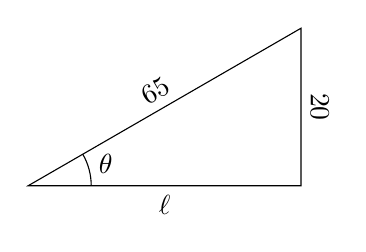
\begin{tikzpicture}[scale=4]
					\draw (0,0) -- node[below] {$ \ell $} (0,0-|30:1) -- node[rotate=-90,above] {\SI{20}{\meter}} (30:1) -- node[above,rotate=30] {\SI{65}{\meter}} cycle;
					\draw (0.2,0) arc (0:30:0.2) node[midway, right, yshift=2pt] {$ \theta $};
				\end{tikzpicture}
			\end{multi}

			Achando o volume de areia, temos $ \approx \dfrac{62\cdot 20}{2}\cdot4000=\SI{2480000}{\meter\cubed} $. Supondo que em cada centímetro cúbico de areia temos \num{1.5e4} grãos, há
			\[ \dfrac{\num{1.5e4}\cdot\num{2.5e6}}{\num{1e-9}}\approx\num{3.75e19}\ \text{grãos de areia} \]
		\end{solution}
		\part o número de átomos contidos num grão de areia.

		\begin{solution}
			Estimando que um átomo de silício tenha $ D=\SI{1e-10}{\meter} $ de diâmetro, se há 100 grãos de areia em \SI{1}{\milli\meter\cubed} de qualquer porção na praia, há $ \sqrt[3]{100}\approx \num{4.6}\ $grãos de areia por milímetro (em fileira). Sendo assim, cada grão tem $ d=\SI{0.22}{\milli\meter} $ de diâmetro. Aproximando um grão de areia e um átomo por esferas perfeitas, teremos
			\begin{align*}
				\dfrac{V_{\text{Areia}}}{V_{\text{Silício}}} & =\dfrac{\cancel{\dfrac{4}{3}\pi} \del{\dfrac{D}{2}}^{3}}{\cancel{\dfrac{4}{3}\pi}\del{\dfrac{d}{2}}^{3}}=\dfrac{\dfrac{D^{3}}{\cancel{2^{3}}}}{\dfrac{d^{3}}{\cancel{2^{3}}}} \\
				                                             & =\del{\dfrac{D}{d}}^{3}=\del{\dfrac{\num{0.22e-3}}{\num{1e-10}}}^{3}\approx\num{1.06e19}
			\end{align*}
			átomos de silício por grão de areia.
		\end{solution}
	\end{parts}

	\question
	A sonda cosmológica WMAP (\textit{Wilkinson Microwave Anisotropy Probe}) determinou em 2014 que a densidade média de átomos no Universo é equivalente a 1 próton por \SI{4}{\kilo\meter\cubed}.

	\begin{parts}
		\part Estime a massa total contida dentro do raio do Universo;

		\begin{solution}
			Estimando o raio do Universo observável em \SI{46e9}{\lightyear}, sendo que a luz viaja no vácuo há $ \approx\SI{3e8}{\meter\per\second} $. Como um ano tem $ \approx \SI{\pi e7}{\second} $, temos $ \num{3e8}\cdot\num{\pi e7}\cdot\num{46e9}\approx\SI{4.3e26}{\meter} $ de raio o Universo (em metros). Supondo um Universo esférico e homogêneo, temos \[  V=\dfrac{4}{3}\pi\num{4.3e26}\approx\SI{3.33e80}{\meter\cubed}\Rightarrow m=V\cdot d\cdot m_p=\num{3.33e80}\cdot\num{0.25}\cdot \num{1.67e-27} \approx \SI{1.39e53}{\kilo\gram} \] onde $ m_p=\SI{1.67e-27}{\kilo\gram} $ é a massa do próton
		\end{solution}
		\part Estime o número total de núcleons (nêutrons e prótons) contido nesse volume;

		\begin{solution}
			Estimando quantidades iguais de nêutrons e prótons, os quais possuem praticamente a mesma massa ($ m_p=\SI{1.67e-27}{\kilo\gram} $), temos, aproximadamente, $ \dfrac{\num{2.2e54}}{2\cdot\num{1.67e-27}}\approx\num{6,6e80}\ \text{nuclêons} $.
		\end{solution}

		\part Compare a densidade média de matéria no Universo com a densidade típica do interior do núcleo atômico.

		\begin{solution}
			Sendo a densidade média do núcleo atômico estimada em \SI{2.4e17}{\kilo\gram\per\meter\cubed}, ela é cerca de \num{5.7e44} vezes maior que a densidade média do Universo.
		\end{solution}
	\end{parts}

	\question

	Considere uma estrela que sofre algum tipo de oscilação. Como a frequência $ \omega $ da oscilação depende das propriedades da estrela?
	Como sempre o primeiro passo é identificar as variáveis físicas relevantes.
	Discuta porque aqui as variáveis relevantes são a densidade de massa $ \rho $, o raio da estrela $ R $ e a constante $ \mathrm{G} $ da lei da gravitação universal de Newton.
	Considere que a densidade de massa possa ser considerada aproximadamente constante. Use análise dimensional para encontrar a dependência de $ \omega $ com as propriedades da estrela.

	\begin{solution}

		\begin{multi}
			Fazendo $ \sbr{\rho}^{\alpha} \sbr{R}^{\beta} \sbr{\mathrm{G}}^{\gamma}=\sbr{\omega} $, onde
			\begin{align*}
				\sbr{\rho}       & =\dfrac{M}{L^{3}}      \\
				\sbr{R}          & =L                     \\
				\sbr{\mathrm{G}} & =\dfrac{L^{3}}{MT^{2}} \\
				\sbr{\omega}     & =T^{-1}
			\end{align*}
			portanto: \begin{align*}
				\del{\dfrac{M}{L^{3}}}^{\alpha}\del{L}^{\beta}\del{\dfrac{L^{3}}{MT^{2}}}^{\gamma} & =T^{-1} \\
				M^{\alpha-\gamma}\cdot L^{-3\alpha+\beta+3\gamma}\cdot T^{-2\gamma}                & =T^{-1}
			\end{align*}

			\nextcol

			Daí, temos que
			\[ \begin{cases}
					\alpha-\gamma=0          \\
					\beta+3(\gamma-\alpha)=0 \\
					-2\gamma=-1
				\end{cases} \]
			e, portanto
			\[ \begin{cases}
					\gamma=1/2                        \\
					\alpha-1/2=0\implies\alpha=1/2    \\
					\beta+3(1/2-1/2)=0\implies\beta=0 \\
				\end{cases} \]
			e, então, temos a expressão final $ k\rho^{1/2}\,\mathrm{G}^{1/2}=\omega\implies \omega=k\sqrt{\rho\,\mathrm{G}} $ onde $ k\in\mathbb{R} $ é uma constante.
		\end{multi}
	\end{solution}

	\question
	Considere ondas na superfície da água, que são chamada de ondas de gravidade.
	Como a frequência $ \omega $ dessas ondas depende do chamado número de onda $ k $?
	Discuta porque as quantidades relevantes aqui são a densidade da água $ \rho $, a aceleração da gravidade $ g $ e $ k $.
	Use o fato que $ \sbr{k}=L^{-1} $ e análise dimensional para encontrar $ \omega\del{k} $.

	\begin{solution}

		\begin{multi}
			Fazendo $ \sbr{k}^{\alpha} \sbr{\rho}^{\beta} \sbr{g}^{\gamma}=\sbr{\omega} $, onde
			\begin{align*}
				\sbr{k}      & =L^{-1}           \\
				\sbr{\rho}   & =\dfrac{M}{L^{3}} \\
				\sbr{g}      & =\dfrac{L}{T^{2}} \\
				\sbr{\omega} & =T^{-1}
			\end{align*}
			portanto: \begin{align*}
				\del{L^{-1}}^{\alpha}\del{\dfrac{M}{L^{3}}}^{\beta}\del{\dfrac{L}{T^{2}}}^{\gamma} & =T^{-1} \\
				L^{-\alpha-3\beta+\gamma}\cdot M^{\beta}\cdot T^{-2\gamma}                         & =T^{-1}
			\end{align*}

			\nextcol

			Daí, temos que
			\[ \begin{cases}
					-\alpha-3\beta+\gamma=0 \\
					\beta=0                 \\
					-2\gamma=-1
				\end{cases} \]
			e, portanto
			\[ \begin{cases}
					\gamma=1/2                              \\
					\beta=0                                 \\
					-\alpha-3\cdot0+1/2=0\implies\alpha=1/2 \\
				\end{cases} \]
			e, então, temos a expressão final $ c\,k^{1/2}\,g^{1/2}=\omega\implies \omega=c\sqrt{k\,g} $ onde $ c\in\mathbb{R} $ é uma constante.
		\end{multi}

	\end{solution}

	\question

	Em explosões nucleares há essencialmente uma liberação instantânea de energia $ E $ em uma pequena região do espaço.
	Isso produz uma onda de choque esférica, com a pressão dentro da onda de choque milhares de vezes maior que a pressão inicial do ar.
	Como o raio $ R $ da onda de choque cresce com o tempo $ t $?
	Discuta por que as quantidades relevantes são $ E $, $ t $ e a densidade do ar $ \rho $.
	Use análise dimensional para obter $ R\del{t} $.
	Em 1950 as fotografias do projeto Trinity foram divulgadas pelo governo americano e publicadas na revista \textit{Life}.
	Usando essas fotografias (tiradas em tempos sucessivos após a explosão nuclear) e a mesma análise dimensional feita aqui, o físico britânico G. I. Taylor (Proc. Roy. Soc. London A 200, 235-247, 1950) estimou a energia liberada pela explosão em 22 quilotoneladas de TNT.
	Essa informação na época era considerada confidencial!

	\begin{solution}

		\correctspacing
		\begin{multi}
			Fazendo $ \sbr{E}^{\alpha} \sbr{t}^{\beta} \sbr{\rho}^{\gamma}=\sbr{R} $, onde
			\begin{align*}
				\sbr{E}    & =\dfrac{ML^{2}}{T^{2}} \\
				\sbr{t}    & =T                     \\
				\sbr{\rho} & =\dfrac{M}{L^{3}}      \\
				\sbr{R}    & =L
			\end{align*}
			portanto: \begin{align*}
				\del{\dfrac{ML^{2}}{T^{2}}}^{\alpha}\del{T}^{\beta}\del{\dfrac{M}{L^{3}}}^{\gamma} & =L \\
				M^{\alpha+\gamma}\cdot L^{2\alpha-3\gamma}\cdot T^{-2\alpha+\beta}                 & =L
			\end{align*}

			\nextcol

			Daí, temos que
			\[ \begin{cases}
					\alpha+\gamma=0   \\
					2\alpha-3\gamma=1 \\
					-2\alpha+\beta=0
				\end{cases} \]
			e, portanto
			\[ \begin{cases}
					\alpha=-\gamma                                            \\
					2(-\gamma)-3\gamma=1\implies\gamma=-1/5\implies\alpha=1/5 \\
					\beta=2\cdot(1/5)=2/5                                     \\
				\end{cases} \]
			e, então, temos a expressão final $ k\,E^{1/5}\, t^{2/5}\, \rho^{-1/5}=R(t)\implies R(t)=k\sqrt[5]{\dfrac{E\,t^{2}}{\rho}} $ onde $ k\in\mathbb{R} $ é uma constante.
		\end{multi}

	\end{solution}

	\question
	Dados os vetores: $ \vec{A}=2\ihat-3\jhat+7\khat $ e $ \vec{B}=5\ihat+\jhat+2\khat $, encontre:

	\begin{parts}
		\part $ \vec{A} +{}\vec{B} $
		\begin{solution}
			\begin{align*}
				\vec{A}+{}\vec{B} & =\del{2\ihat+5\ihat}+\del{-3\jhat+\jhat}+\del{7\khat+2\khat} \\
				                  & =\ihat\del{2+5}+\jhat\del{-3+1}+\khat\del{7+2}               \\
				                  & =7\ihat-2\jhat+9\khat
			\end{align*}
		\end{solution}

		\clearpage

		\part $ \vec{A}-{}\vec{B} $

		\begin{solution}
			\begin{align*}
				\vec{A}-{}\vec{B} & =\del{2\ihat-5\ihat}+\del{-3\jhat-\jhat}+\del{7\khat-2\khat} \\
				                  & =\ihat\del{2-5}+\jhat\del{-3-1}+\khat\del{7-2}               \\
				                  & =-3\ihat-4\jhat+5\khat
			\end{align*}
		\end{solution}

		\part $ \vec{A} \cdot \vec{B} $

		\begin{solution}
			\begin{align*}
				\vec{A}\cdot\vec{B} & =\<(2,-3,7),(5,1,2)>        \\
				                    & =2\cdot5+(-3)\cdot1+7\cdot2 \\
				                    & =10-3+14=21
			\end{align*}
		\end{solution}

		\part o valor de $ \envert{\vec{A}}\equiv A \equiv \sqrt{\vec{A}\cdot \vec{A}}=\sqrt{\vec{A}^{2}} $ e de
		$ \envert{\vec{B}}\equiv B \equiv \sqrt{\vec{B}\cdot \vec{B}}=\sqrt{\vec{B}^{2}} $

		\begin{solution}
			\begin{align*}
				\<\vec{A},\vec{A}> & =\<(2,-3,7),(2,-3,7)>=2^{2}+(-3)^{2}+7^{2}=4+9+49=62\implies\sqrt{\<\vec{A},\vec{A}>}=\sqrt{62} \\
				\<\vec{B},\vec{B}> & =\<(5,1,2),(5,1,2)>=5^{2}+1^{2}+2^{2}=25+1+4=30\implies\sqrt{\<\vec{B},\vec{B}>}=\sqrt{30}
			\end{align*}
		\end{solution}

		\part o cosseno do ângulo entre $ \vec{A} $ e $ \vec{B} $

		\begin{solution}
			Sendo $\envert{\vec{A}}=\sqrt{62}$ e $\envert{\vec{B}}=\sqrt{30}$, $\vec{A}\cdot\vec{B}=|\vec{A}||\vec{B}|\cos\theta=\<(2,-3,7),(5,1,2)>=21$, onde $\theta$ é o ângulo entre os vetores.
			Resolvendo para $ \theta $, temos
			\[ 21=\sqrt{62}\ \sqrt{30}\cos\theta\implies\theta=\arccos{\del{\dfrac{21}{2\sqrt{31\cdot5\cdot3}}}} \]
		\end{solution}

		\part $ \vec{A}\times\vec{B} $

		\begin{solution}
			\begin{align*}
				\vec{A}\times\vec{B} & =\begin{vmatrix}
					\ihat & \jhat & \khat \\
					2     & -3    & 7     \\
					5     & 1     & 2
				\end{vmatrix}=\ihat\begin{vmatrix}
					-3 & 7 \\
					1  & 2
				\end{vmatrix} - \jhat\begin{vmatrix}
					2 & 7 \\
					5 & 2
				\end{vmatrix} + \khat\begin{vmatrix}
					2 & -3 \\
					5 & 1
				\end{vmatrix} \\
				                     & =\ihat\del{-6-7}-\jhat\del{4-35}+\khat\del{2+15}                                                                                \\
				                     & =(-13,31,17)
			\end{align*}
		\end{solution}
	\end{parts}

	\clearpage

	\question
	Mostre

	\begin{parts}
		\part que se $ \envert{\vec{C}-\vec{D}}=\envert{\vec{C}+\vec{D}} $, então $ \vec{C} $ é um vetor perpendicular a $\vec{D}$;

		\begin{solution}
			Fazendo $\sqrt{(\vec{C}-\vec{D})(\vec{C}-\vec{D})}=\sqrt{(\vec{C}+\vec{D})(\vec{C}-\vec{D})}$ temos
			\begin{align*}
				\cancel{\vec{C}\cdot \vec{C}}-2\vec{C}\cdot \vec{D}+\cancel{\vec{D}\cdot\vec{D}} & =\cancel{\vec{C}\cdot\vec{C}}+2\vec{C}\cdot\vec{D}+\cancel{\vec{D}\cdot\vec{D}}\Leftrightarrow \\
				-\cancel{2}\vec{C}\cdot\vec{D}                                                   & =\cancel{2}\vec{C}\cdot\vec{D}\Leftrightarrow                                                  \\
				-\cancel{C\ D}\cos\theta                                                         & =\cancel{C\ D}\cos\theta\Leftrightarrow                                                        \\
				-\cos\theta                                                                      & =\cos\theta
			\end{align*}
			Portanto,
			\[ \cos\theta=0\implies\theta=\SI{\pi/2}{\radian} \text{ ou }\theta=\SI{3\pi/2}{\radian} \]
			e então os vetores devem ser perpendiculares.

			\hfill\qedsymbol
		\end{solution}

		\part a lei dos senos considerando a área de um triângulo formado pelos vetores $\vec{a}$, $\vec{b}$ e $\vec{c}$, onde $\vec{a} + \vec{b} + \vec{c} = 0$;

		\begin{solution}

			%			\correctspacing
			\begin{multi}
				Seja o triângulo de lados $ a=|\vec{a}|,b=|\vec{b}|,c=|\vec{c}| $ e ângulos $ \alpha,\beta,\gamma $ apostos aos lados $ a,b $ e $ c $, respectivamente. Pelo produto vetorial, a área $ A $ desse triângulo é igual à:
				\[ A=\dfrac{1}{2}|\vec{a}\times\vec{b}|=\dfrac{1}{2}|\vec{b}\times\vec{c}|=\dfrac{1}{2}|\vec{c}\times\vec{a}| \]

				\nextcol

				\centering
				\begin{tikzpicture}[scale=2]
					\coordinate (A) at (0,0);
					\coordinate (B) at (30:2);
					\coordinate (C) at (3,0);

					\draw (A) -- node[above left] {$ a $} (B) -- node[above right] {$ b $} (C) -- node[below] {$ c $} cycle;

					\pic[draw=black, angle radius=10pt,angle eccentricity=1,"$ \gamma $" {shift={(-1pt,-5pt)}}] {angle=A--B--C};

					\pic[draw=black, angle radius=15pt,angle eccentricity=1,"$ \alpha $" {shift={(-5pt,2pt)}}] {angle=B--C--A};

					\pic[draw=black, angle radius=15pt,angle eccentricity=1,"$ \beta $" {shift={(5pt,1pt)}}] {angle=C--A--B};
				\end{tikzpicture}
			\end{multi}



			Logo, valem as igualdades
			\begin{align}
				\dfrac{1}{2}a\,b\sin\gamma=\dfrac{1}{2}b\,c\sin\alpha\implies \dfrac{a}{\sin\alpha}=\dfrac{c}{\sin\gamma} \\
				\dfrac{1}{2}a\,b\sin\gamma=\dfrac{1}{2}c\,a\sin\beta\implies \dfrac{b}{\sin\beta}=\dfrac{c}{\sin\gamma}   \\
				\dfrac{1}{2}b\,c\sin\alpha=\dfrac{1}{2}c\,a\sin\beta\implies \dfrac{b}{\sin\beta}=\dfrac{a}{\sin\alpha}
			\end{align}

			\hfill\qedsymbol
		\end{solution}

		\clearpage

		\part que se $\hat{a}$ e $\hat{b}$ são vetores unitários (versores) no plano $x\,y$ fazendo um 	ângulo $ \theta $ e $ \phi $ com o eixo $ x $, respectivamente, então esses versores 	podem ser representados como $ \hat{a}=\cos\theta\ihat+\sin\theta\jhat $ e $ \hat{b}=\cos\phi\ihat+\sin\phi\jhat $.
		Use isso para provar que $ \cos{\del{\theta-\phi}}=\cos\theta\cos\phi+\sin\theta\sin\phi $.

		\begin{solution}
			\begin{multi}
				Desenhando um diagrama genérico para a situação temos a figura ao lado.

				\nextcol

				\begin{tikzpicture}[scale=3]
					\draw[->] (-0.25,0) -- (1.25,0) node[right] {$ x $};
					\draw[->] (0,-0.25) -- (0,1.25) node[above] {$ y $};

					\coordinate (x) at (1,0);
					\coordinate (O) at (0,0);
					\coordinate (b) at (30:1);
					\coordinate (a) at (60:1);

					\draw[-Latex] (0,0) -- node[rotate=60,above] {$ \hat{a} $} (a);
					\draw[-Latex] (0,0) -- node[rotate=30,above] {$ \hat{b} $} (b);

					\pic[->,draw=black, angle radius=30pt,angle eccentricity=1,"$ \phi $" {shift={(5pt,2pt)}}] {angle=x--O--b};

					\pic[->,draw=black, angle radius=20pt,angle eccentricity=1,"$ \theta $" {shift={(2pt,8pt)}}] {angle=x--O--a};
				\end{tikzpicture}
			\end{multi}

			\begin{multi}
				Podemos decompor o vetor $\hat{a}$ usando o ângulo $\theta$ formado com o eixo $ x $:
				\[ \begin{cases}
						a_x=\hat{a}\cdot\ihat=1\cdot1\cdot\cos\theta=\cos\theta \\
						a_y=\hat{a}\cdot\jhat=1\cdot1\cdot\cos{(\ang{90}-\theta)}=\sin\theta
					\end{cases} \]
				Portanto, temos \[ \hat{a}=\vec{a_x}+\vec{a_y}=\cos\theta\ihat+\sin\theta\jhat \]
				\paragraph{Nota:} $ \cos{\del{\ang{90}-\theta}}=\sin{\theta} $ pela definição de $ \sin\theta $ e $ \cos\theta $ num triângulo retângulo.
				\nextcol
				\begin{tikzpicture}[scale=3]
					\draw[->] (-0.25,0) -- (1.25,0) node[right] {$ x $};
					\draw[->] (0,-0.25) -- (0,1.25) node[above] {$ y $};

					\coordinate (x) at (1,0);
					\coordinate (O) at (0,0);
					\coordinate (b) at (30:1);
					\coordinate (a) at (60:1);

					\draw[-Latex] (0,0) -- node[rotate=60,above] {$ \hat{a} $} (a);

					\pic[->,draw=black, angle radius=20pt,angle eccentricity=1,"$ \theta $" {shift={(4pt,3pt)}}] {angle=x--O--a};

					\draw[dashed] (a|-0,0) coordinate (ax) -- (a);
					\draw[dashed] (a-|0,0) coordinate (ay) -- (a);
				\end{tikzpicture}
			\end{multi}

			\begin{multi}
				Utilizando raciocínio análogo para $\hat{b}$, temos:
				\[ \hat{b}=\vec{b_x}+\vec{b_y}=\cos\phi\ihat+\sin\phi\jhat \]
				\nextcol
				\begin{tikzpicture}[scale=3]
					\draw[->] (-0.25,0) -- (1.25,0) node[right] {$ x $};
					\draw[->] (0,-0.25) -- (0,1.25) node[above] {$ y $};

					\coordinate (x) at (1,0);
					\coordinate (O) at (0,0);
					\coordinate (b) at (30:1);
					\coordinate (a) at (60:1);

					\draw[-Latex] (0,0) -- node[rotate=30,above] {$ \hat{b} $} (b);

					\pic[->,draw=black, angle radius=30pt,angle eccentricity=1,"$ \phi $" {shift={(5pt,2pt)}}] {angle=x--O--b};

					\draw[dashed] (b|-0,0) coordinate (bx) -- (b);
					\draw[dashed] (b-|0,0) coordinate (by) -- (b);

				\end{tikzpicture}
			\end{multi}

			Retomando o primeiro diagrama da resolução, temos que \[ \hat{a}\cdot\hat{b}=a\cdot b\cdot\cos{(\theta-\phi)}=a_x\,b_x+a_y\,b_y\implies\cos{(\theta-\phi)}=\cos\theta\cos\phi+\sin\theta\sin\phi \]

			\hfill\qedsymbol
		\end{solution}
	\end{parts}

	\clearpage

	\question
	Considere dois pontos localizados em $r_1$ e $r_2$ e separados pela distância $ r=\envert{r_1-r_2} $.
	Encontre o vetor $\vec{A}$ da origem até um ponto na reta que liga $r_1$ a $r_2$ a uma distância $ xr $ do ponto $ r_1 $, onde $ x $ é algum número.

	\begin{solution}

		\begin{multi}
			O vetor pode ser descrito por $ \vec{A}=\overline{Or_1}+x\overline{r_1r_2\vphantom{O}} $ que é o segmento da origem do plano $ O $ até $ r_1 $, e então somado ao segmento que vai de $ r_1 $ a $ r_2 $ multiplicado por $ x\in\mathbb{R} $.
			\nextcol
			\begin{tikzpicture}[scale=2]
				\draw[->] (-0.5,0) -- (2,0) node[right] {$ x $};
				\draw[->] (0,-0.5) -- (0,2) node[above] {$ y $};

				\coordinate (r1) at (30:1.5);
				\coordinate (r2) at (60:1.7);

				\filldraw (r1) circle (1pt) node[above right] {$ r_1 $} -- (r2) circle (1pt) node[above right] {$ r_2 $};

				\coordinate (r) at ($ (r2)-(r1) $);
				\coordinate (rf) at ($ (r2)+(0,0)!0.5!(r) $);

				\draw[dashed] (r1) -- (rf);
				\draw[-Latex] (0,0) -- node[rotate=70,above] {$ \vec{A} $} (rf);
				\draw[decorate,decoration={brace,amplitude=10pt,mirror,raise=4pt}] ($ (r1)!0.25cm!-90:(rf) $) -- node[rotate=-60,shift={(90:20pt)}] {$ xr $} ($ (rf)!0.25cm!90:(r1) $);
			\end{tikzpicture}
		\end{multi}

	\end{solution}

	\question
	Seja $\vec{A}$ um vetor arbitrário e seja $\hat{n}$ um versor em alguma direção fixa.
	Mostre que sempre podemos escrever $\vec{A}$ como a soma de dois vetores: um na direção de $\hat{n}$ e outro na direção perpendicular.
	Ou seja, que \[ \vec{A} = (\vec{A} \cdot \hat{n}) \hat{n} + (\hat{n} \times \vec{A}) \times \hat{n} \]

	\by{Anahí}
	\begin{solution}

		\begin{multi}
			Imaginemos a situação ao lado:

			\smallskip

			Como $ |\vec{A_n}|=\vec{A}\cdot\hat{n} $ e $ |\vec{A_r}|=\vec{A}\cdot\hat{r} $ então, teremos
			\begin{align*}
				\vec{A} & =\vec{A_{n}}+\vec{A_{r}}                                                                                                                   \\
				        & =|\vec{A_n}|\hat{n}+|\vec{A_r}|\hat{r}                                                                                                     \\
				        & =\del{\vec{A}\cdot\hat{n}}\hat{n}+\del{\hat{r}\cdot\vec{A}}\hat{r}                                                                         \\
				        & =\del{\vec{A}\cdot\hat{n}}\hat{n}+\del{\underbrace{|\hat{r}|}_{=|\hat{n}|}|\vec{A}|\underbrace{\cos{(\pi/2-\theta)}}_{=\sin\theta}}\hat{r} \\
				        & =\del{\vec{A}\cdot\hat{n}}\hat{n}+\del{|\hat{n}||\vec{A}|\sin\theta}\hat{r}                                                                \\
				        & =\del{\vec{A}\cdot\hat{n}}\hat{n}+\del{|\hat{n}\times\hat{A}|}\hat{r}
			\end{align*}

			\nextcol

			\centering
			\begin{tikzpicture}[scale=2]
				%			\draw[->] (-0.5,0) -- (2,0) node[right] {$ x $};
				%			\draw[->] (0,-0.5) -- (0,2) node[above] {$ y $};

				\draw[-Latex,blue] (0,0) -- (1.5,0) node[below,blue,very near end] {$ \vec{A_{n}} $};
				\draw[-Latex,blue] (0,0) -- (0,1.5) node[left,blue,very near end] {$ \vec{A_{r}} $};

				\draw[-Latex,red] (0,0) -- node[above,red,near end] {$ \hat{n} $} (1,0);
				\draw[-Latex,red] (0,0) -- node[right,red] {$ \hat{r} $} (0,1) coordinate (r);
				\draw[-Latex,red] (xyz cs:z=0) -- node[above,red] {$ \hat{\gamma} $} (xyz cs:z=1) coordinate (g);

				\draw[-Latex,blue] (0,0) -- node[rotate=45,above,blue] {$ \vec{A} $} (1.5,1.5);

				\draw[dashed] (1.5,0) -- (1.5,1.5) -- (0,1.5);

				\coordinate (A) at (1.5,1.5);
				\coordinate (O) at (0,0);
				\coordinate (n) at (1.5,0);

				\pic[draw=black,fill=gray!50, angle radius=20pt,angle eccentricity=1,"$ \theta $" {xshift=5pt,yshift=0pt}] {angle=n--O--A};

				\draw (xyz cs:z=0pt,y=0.2) -- ++(xyz cs:z=0.2) -- +(xyz cs:y=-0.2);
				\draw (xyz cs:z=0pt,x=0.2) -- ++(xyz cs:z=0.2) -- +(xyz cs:x=-0.2);
				\node[circle,fill,inner sep=.5pt] at (xyz cs:z=0.1,y=0.1) {};
				\node[circle,fill,inner sep=.5pt] at (xyz cs:z=0.1,x=0.1) {};
			\end{tikzpicture}
		\end{multi}

		Seja $\hat{\gamma}$ um vetor saindo do plano do papel, no sentido de $ \hat{n}\times\hat{r}=\hat{n}\times\hat{A} $.
		Podemos notar que $ \hat{\gamma}\times\hat{n} $ estará na mesma direção e sentido de $\hat{r}$ (pela regra da mão direita). Como o módulo $ |\hat{n}\times\hat{A}| $ é preservado no produto vetorial, temos:

		\[ \vec{A}=\del{\vec{A}\cdot\hat{n}}\hat{n}+\del{\hat{n}\times\vec{A}}\times\hat{n} \]

	\end{solution}

\end{questions}
\end{document}
